
\begin{figure}
\centering
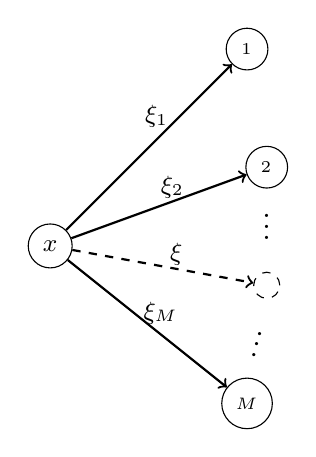
\begin{tikzpicture}

\draw (.5,.5) node(ROOT)[circle,draw]{\small $x$ };
\draw (3,3) node(ONE)[circle,draw]{ \small $\cX_1$ };
\draw (3.25,1.5) node(TWO)[circle,draw]{ \small $\cX_2$ };
\draw (3.25,.85) node(DOTONE){ \large $\vdots$ };
\draw (3.25,0) node(N)[circle,dashed,draw]{ \small $\cX$ };
\draw (3.15,-.65) node(DOTTWO)[rotate=-15]{ \large $\vdots$ };
\draw (3,-1.5) node(S)[circle,draw]{ \small $\cX_M$ };

\draw (1.85,2.15) node(OMG1){ \small $\xi_1$ };
\draw (2.05,1.25) node(OMG2){ \small $\xi_2$ };
\draw (2.1,.4) node(OMG){ \small $\xi$ };
\draw (1.9,-.35) node(OMGS){ \small $\xi_M$ };

\draw[thick, ->] (ROOT) -- (ONE) ;
\draw[thick,->] (ROOT) -- (TWO);
\draw[thick,dashed, ->] (ROOT) -- (N);
\draw[thick,->] (ROOT) -- (S);

%\draw[thick,dashed] (TWO) -- (N);
%\draw[thick,dashed] (N) -- (S);

\end{tikzpicture} 
\caption{Scenario Tree for Two Stage Problem}
  \label{fig:mip}
\end{figure}
